\documentclass[12pt]{article}

\usepackage[spanish]{babel}

\usepackage{amsmath}
\usepackage{amssymb}

\usepackage{hyperref}
\usepackage{graphicx}
\usepackage{listings}
\usepackage{color}
\usepackage{multicol}
\usepackage{enumitem}
\usepackage{here}
\usepackage{dsfont}
\usepackage{tipa}
\usepackage{float}
\usepackage{dsfont} 
\spanishdecimal{.}

\title{Matemáticas para las Ciencias Aplicadas II}
\title{
	\textbf{Tarea 01} \\
	\vspace{1ex}
	\large Matemáticas para las Ciencias Aplicadas II \\
	Facultad de Ciencias, UNAM}
\date{\today}
\author{Flores Morán Julieta Melina \\ Zarco Romero José Antonio}

\begin{document}
\maketitle

% 1 -------------------------------------------------------------------------------------------------------------
\section{}

¿Cuáles son las proyecciones del \textbf{punto} $A(2,3,5)$ en los planos \textbf{xy} \textbf{yz} y \textbf{xz}? Para calcular, trace una caja rectangular con vértices en el origen y el punto A como vértices opuestos y con sus caras paralelas a los planos coordenados. Etiquete todos los vértices de la caja. Asimismo calcule la longitud de la diagonal de la caja.

\begin{itemize}
  
\item Trazo de la caja:
  
  \begin{figure}[H]
    \centering
    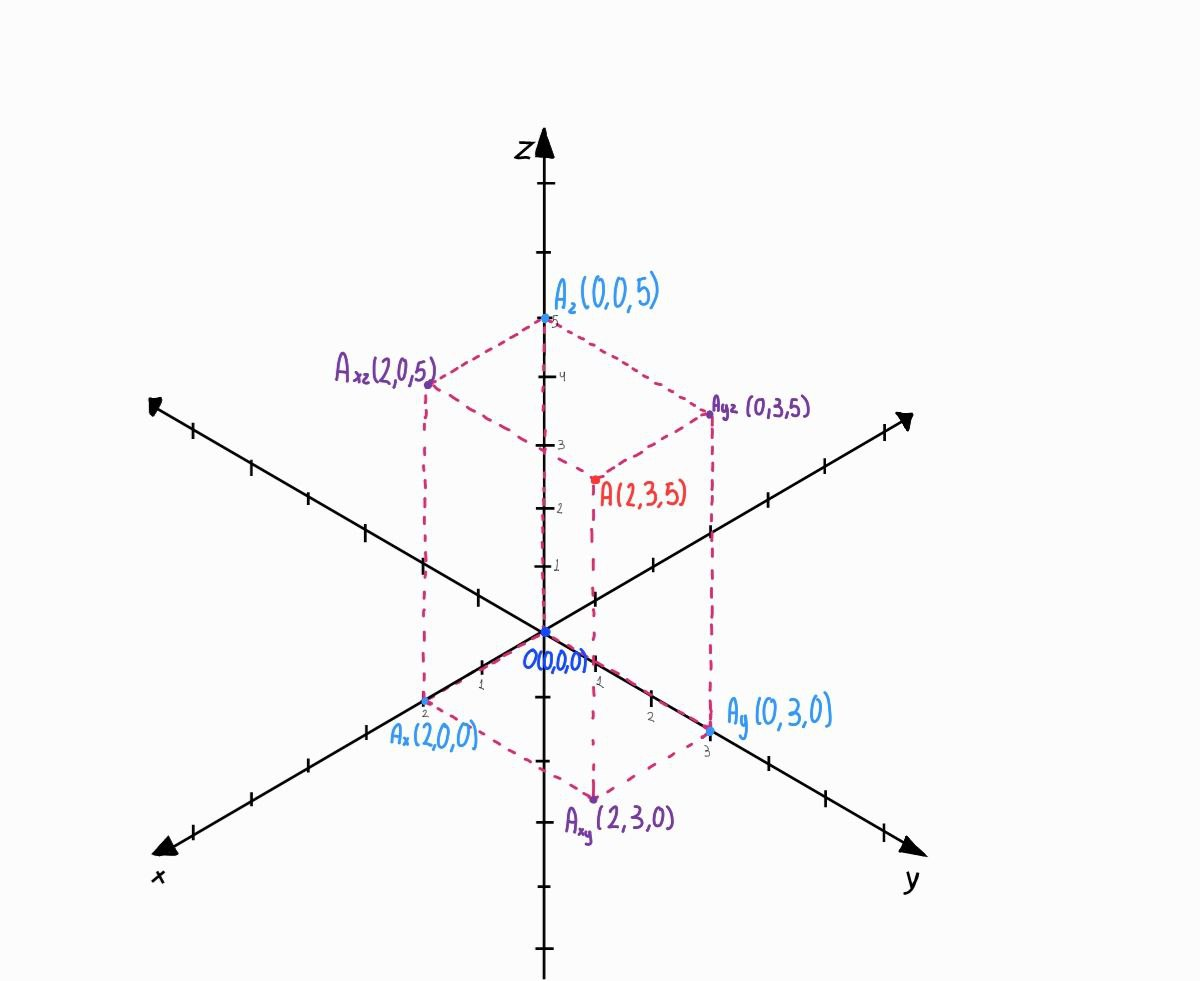
\includegraphics[width=1\textwidth]{./img/caja.jpeg}
  \end{figure}
  
\item Proyecciones del punto:
  \begin{itemize}
    
  \item \textbf{Plano xy:}
    
    En este plano, la coordenada $z=0$. Por lo que el punto sería $A_{xy}(2, 3, 0)$.
     \begin{figure}[H]
    \centering
    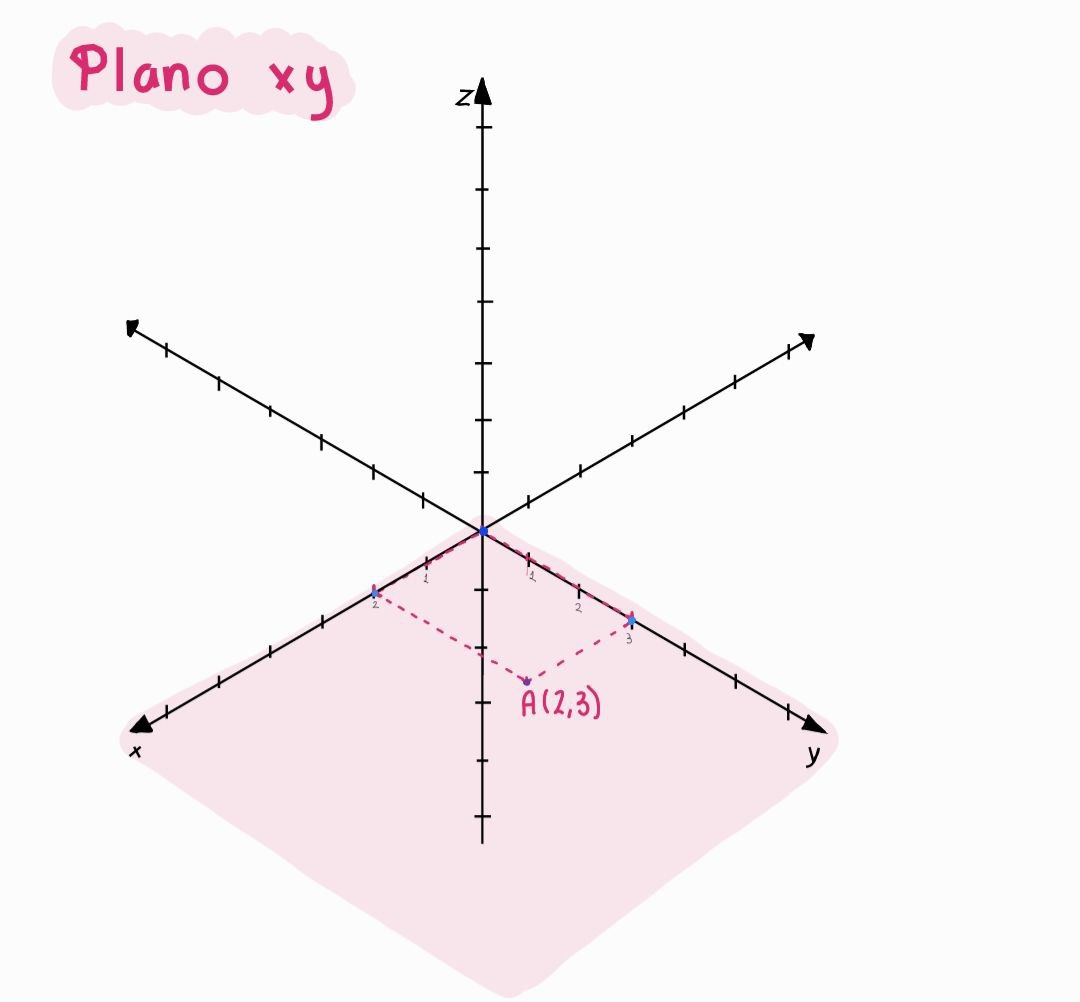
\includegraphics[width=0.5\textwidth]{./img/interxy.jpeg}
     \end{figure}
     
  \item \textbf{Plano yz:}
    
    En este plano, la coordenada $x=0$. Por lo que el punto sería $A_{yz}(0, 3, 5)$.
     \begin{figure}[H]
    \centering
    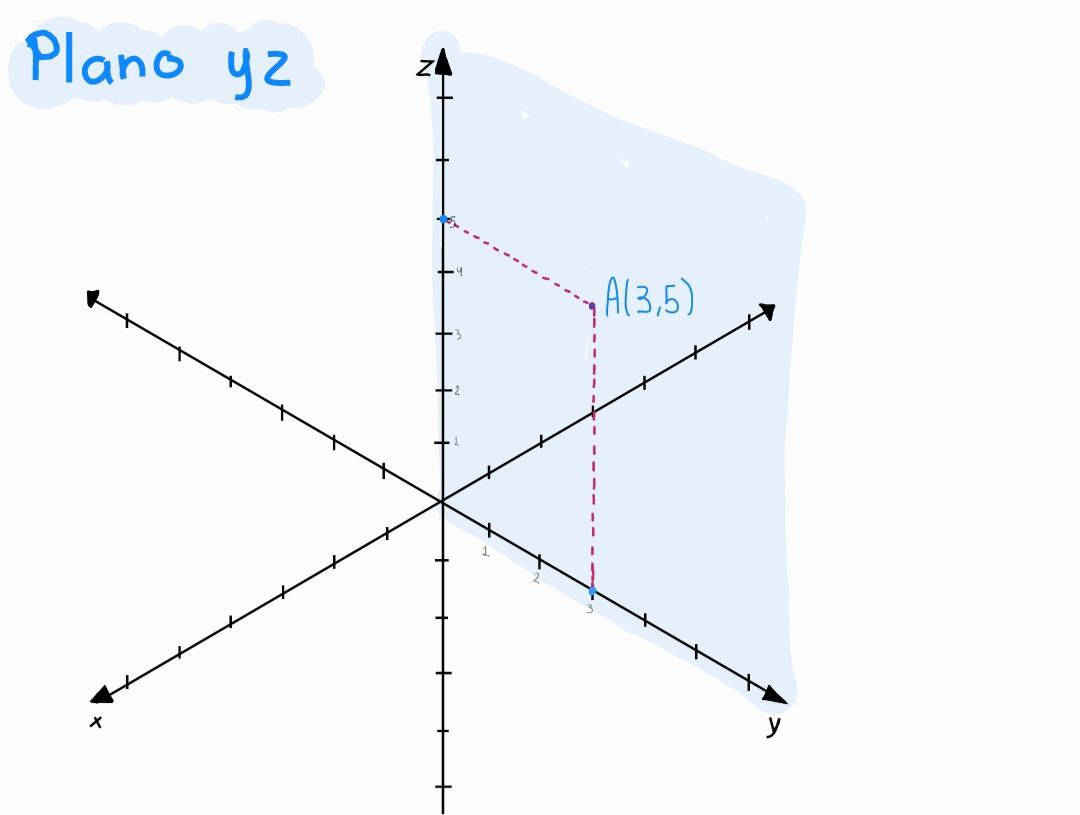
\includegraphics[width=0.5\textwidth]{./img/interyz.jpeg}
  \end{figure}
  \item \textbf{Plano xz:}
    
    En este plano, la coordenada $y=0$. Por lo que el punto sería $A_{xz}(2, 0, 5)$.
     \begin{figure}[H]
    \centering
    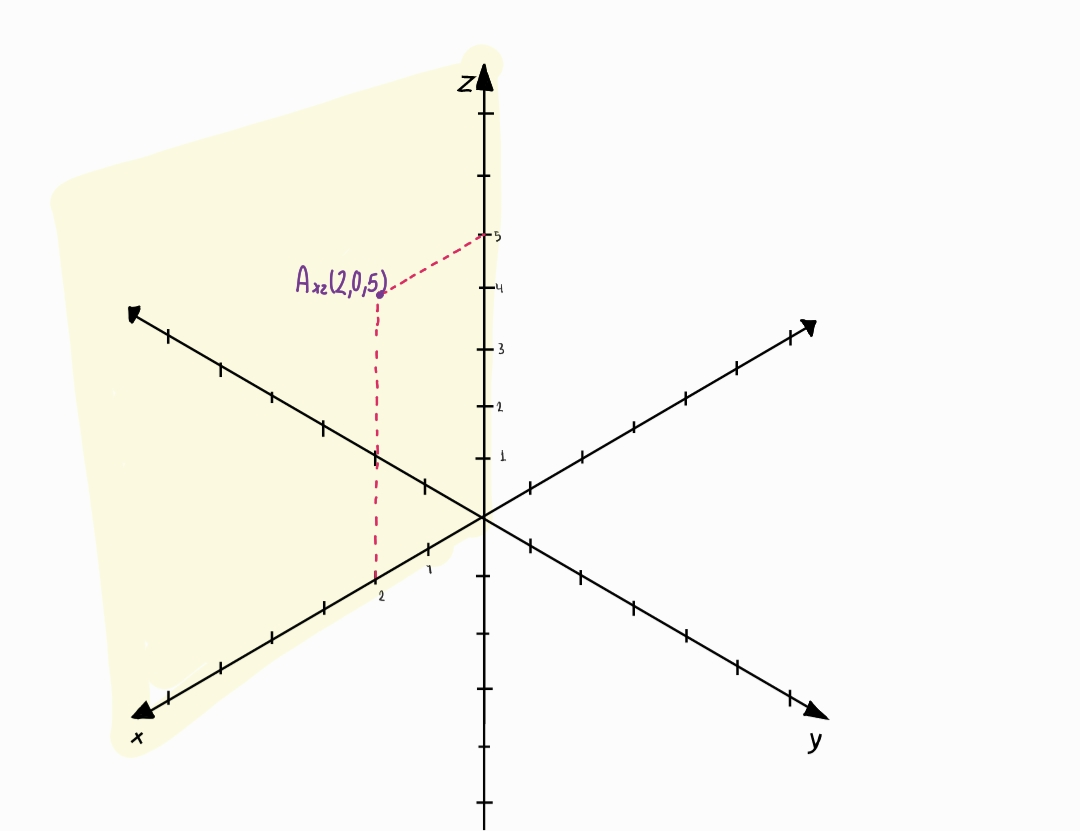
\includegraphics[width=0.5\textwidth]{./img/interxz.jpg}
  \end{figure}
  \end{itemize}
  
\item Longitud de la diagonal de la caja:
  
  La longitud de la diagonal equivale a la norma del vector que va del origen al punto A. Este vector sería $\vec{a} = \vec{OA} = A-O = (2, 3, 5) - (0, 0, 0) = (2,3,5)$.Entonces usamos la fórmula de la norma $||\vec{a}|| = \sqrt{a_x^2 +  a_y^2 + a_z^2}$ y sustituimos $a_x = 2$, $a_y = 3$, $a_z = 5$.
  
  \begin{equation*}
    \begin{split}
      ||\vec{a}|| &= \sqrt{2^2 +  3^2 + 5^2} \\
      &= \sqrt{4 +  9 + 25} \\
      &= \sqrt{38}
    \end{split}
  \end{equation*}
  
  \begin{figure}[H]
    \centering
    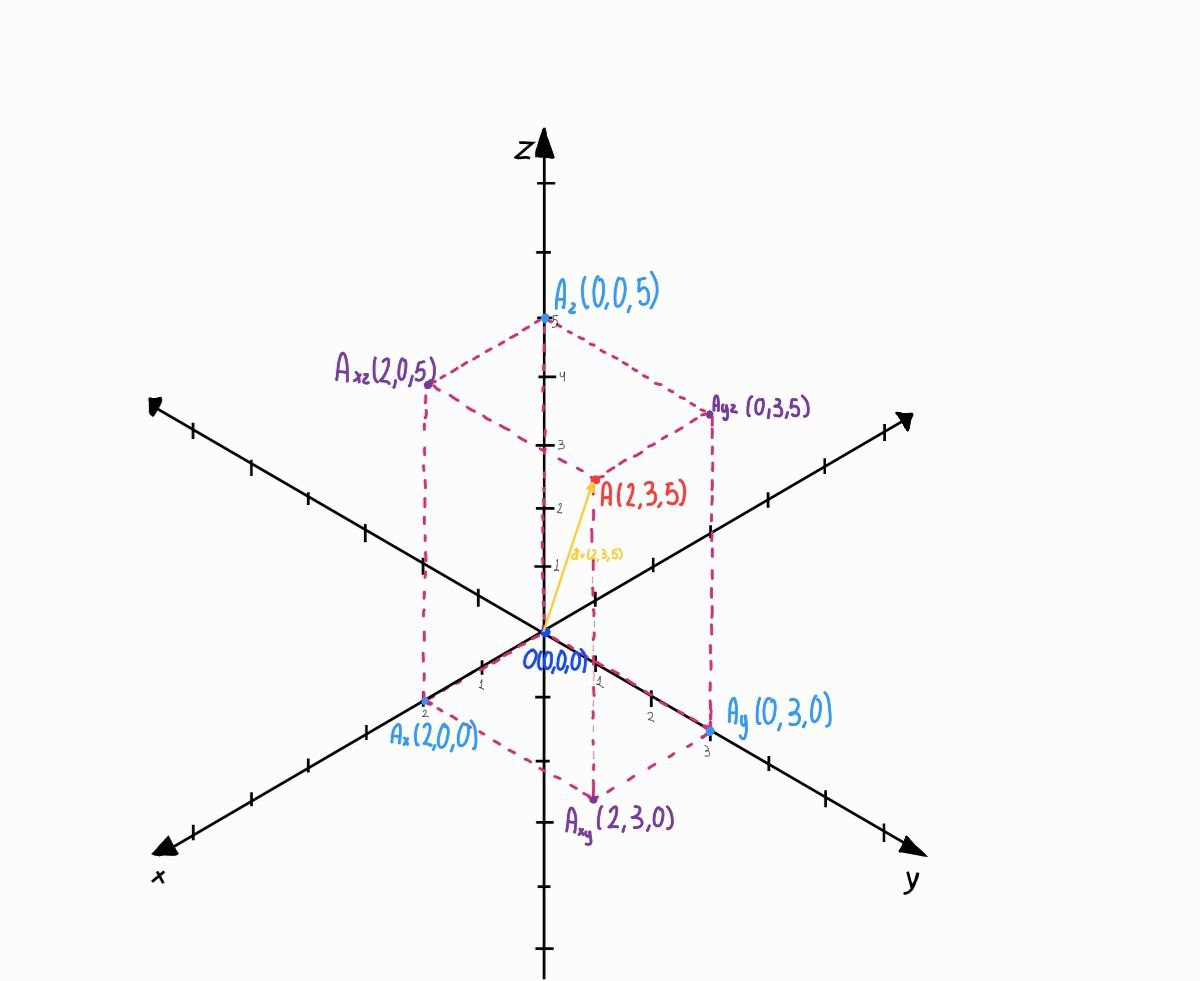
\includegraphics[width=1\textwidth]{./img/diagonal.jpeg}
  \end{figure}
\end{itemize}

% 2 -------------------------------------------------------------------------------------------------------------
\section{}

Determine una ecuación de la esfera que pasa por el origen y cuyo centro es el punto $A(1,2,3)$. Describa su intersección con cada uno de los planos coordenados.\\
Para este ejercicio necesitamos la definición de \textbf{ecuación de la esfera}: La ecuación de la esfera en un sistema de coordenadas cartesianas tridimensional, con centro en el punto (h,j,k) y radio r, se expresa como:
\[
(x-h)^2+(y-j)^2+(z-k)^2=r^2
\]
Donde:
\begin{itemize}
   \item h es la coordenada x del centro de la esfera.
   \item j es la coordenada y del centro de la esfera.
   \item  k es la coordenada z del centro de la esfera.
   \item  r es el radio de la esfera.
\end{itemize}
El radio será la distancia entre los puntos $O(0,0,0)$ (origen) y $A(1,2,3)$ (centro de la esfera), i.e.

\begin{align*}
  r = |OA|
  &= \sqrt{(1-0)^2 + (2-0)^2 + (3-0)^2} \\
  &= \sqrt{1^2 + 2^2 + 3^2} \\
  &= \sqrt{1 + 4 + 9} \\
  &= \sqrt{14}
\end{align*}

Por lo tanto, la ecuación de la esfera es: $$ (x-1)^2 + (y-2)^2 + (z-3)^2 = 14 $$

\begin{enumerate}[format=\textbf]
  
\item Intersección con el plano $xy$.
  
  Sustituimos $z = 0$ en la ecuación de la esfera.
  
  \begin{align*}
    (x-1)^2 + (y-2)^2 + (0-3)^2
    &= 14 \\
    (x-1)^2 + (y-2)^2 + (-3)^2
    &= 14 \\
    (x-1)^2 + (y-2)^2 + 9
    &= 14 \\
    (x-1)^2 + (y-2)^2
    &= 14 - 9 \\
    (x-1)^2 + (y-2)^2
    &= 5 \\
  \end{align*}
  
  Como $z = 0$, los puntos que se encuentran en el plano $xy$ se hallan sobre la circunferencia $(x-1)^2 + (y-2)^2 = 5$.
  
\item Intersección con el plano $xz$.
  
  Sustituimos $y = 0$ en la ecuación de la esfera.
  
  \begin{align*}
    (x-1)^2 + (0-2)^2 + (z-3)^2
    &= 14 \\
    (x-1)^2 + (-2)^2 + (z-3)^2
    &= 14 \\
    (x-1)^2 + 4 + (z-3)^2
    &= 14 \\
    (x-1)^2 + (z-3)^2
    &= 14 - 4 \\
    (x-1)^2 + (z-3)^2
    &= 10 \\
  \end{align*}
  
  Como $y = 0$, los puntos que se encuentran en el plano $xz$ se hallan sobre la circunferencia $(x-1)^2 + (z-3)^2 = 10$.
  
\item Intersección con el plano $yz$.
  
  Sustituimos $x = 0$ en la ecuación de la esfera.
  
  \begin{align*}
    (0-1)^2 + (y-2)^2 + (z-3)^2
    &= 14 \\
    (-1)^2 + (y-2)^2 + (z-3)^2
    &= 14 \\
    1 + (y-2)^2 + (z-3)^2
    &= 14 \\
    (y-2)^2 + (z-3)^2
    &= 14 - 1 \\
    (y-2)^2 + (z-3)^2
    &= 13 \\
  \end{align*}
  
  Como $x = 0$, los puntos que se encuentran en el plano $yz$ se hallan sobre la circunferencia $(y-2)^2 + (z-3)^2 = 13$.
  
\end{enumerate}

% 3 -------------------------------------------------------------------------------------------------------------
\section{}

La siguiente ecuación corresponde a una esfera. Determine las coordenadas del centro y el radio.
\[ x^2 + y^2 + z^2 + 8x - 6y + 2z + 17 = 0 \]

Se puede reescribir la ecuación dada en la forma de la ecuación de una esfera si se completan los cuadrados:

\begin{equation*}
  \begin{split}
    x^2 + y^2 + z^2 + 8x - 6y + 2z + 17 &= 0 \\
    x^2 + 8x + y^2 - 6y + z^2 + 2z + 17 &= 0 \\
    (x^2 + 8x) + (y^2 - 6y) + (z^2 + 2z) &= - 17 \\
    (x^2 + 8x + 16) + (y^2 - 6y + 9) + (z^2 + 2z + 1) &= - 17 + 16 + 9 + 1\\
    (x + 4)^2 + (y - 3)^2 + (z + 1)^2 &= 9 \\
  \end{split}
\end{equation*}

$\therefore $ Se ve que es la ecuación de una esfera con centro $(-4, 3, -1)$ y radio $\sqrt{9} = 3$.

% 4 -------------------------------------------------------------------------------------------------------------
\section{}

Escriba desigualdades para describir las siguientes regiones.

\begin{itemize}
    
\item La región entre el plano \textbf{xz} y el plano vertical \textbf{y=4}.

  Dado que la ecuación del plano $xz$ es $y=0$  y la del plano vertical es $y=4$. La región que delimitan incluye a todos los puntos $(x,y,x)$ donde
  $$0 \leq y \leq 4$$
    
\item La región que consta de todos los puntos entre (pero no sobre) las esferas de radio \textit{r} y \textit{R} centradas en el origen, donde $r < R$.

  Para representar a los puntos $(x,y,z)$ cuya distancia desde el origen es por lo menos $r$, y a lo más, $R$, podemos delimitar a la región como
  $$r < \sqrt{x^2 + y^2 + z^2} < R$$
  o bien,
  $$r^2 < x^2 + y^2 + z^2 < R^2$$
    
\end{itemize}
  
% 5 -------------------------------------------------------------------------------------------------------------
\section{}

Sean $\vec{a} , \vec{b} , \vec{c}$ vectores en $\mathbb{R}^n$ y sean $c,d$ escalares. Escriba las 8 propiedades de los vectores y proporcione una breve explicación de cada una de ellas.

\begin{enumerate}[format=\textbf]

\item $$\vec{a}+\vec{b} = \vec{b}+\vec{a}$$
  
  \textbf{Conmutatividad:} El resultado de sumar dos vectores no depende del orden en el que se toman.

\item $$\vec{a}+\vec{0} = \vec{a}$$
  
  \textbf{Identidad:} El $\vec{0}$ es el elemento neutro de la suma de vectores. Cualquier vector sumado con $\vec{0}$ mantiene su identidad. 

\item $$c(\vec{a}+\vec{b}) = c\vec{a}+c\vec{b}$$
  
   \textbf{Distributividad:} El producto por un escalar se distribuye sobre la suma de vectores, es decir,  multiplicar la suma de dos vectores por un escalar es lo mismo que multiplicar cada vector por el escalar y luego sumar los resultados.

 \item $$(cd)\vec{a} = c(d\vec{a})$$
   
   \textbf{Asociatividad:} El producto entre un vector y escalares es asociativo. Multiplicar un vector por un escalar y luego por otro escalar es lo mismo que multiplicar el vector por el producto de los dos escalares.  

 \item $$\vec{a}+(\vec{b}+\vec{c}) = (\vec{a}+\vec{b})+\vec{c}$$
   
   \textbf{Asociatividad:} La suma de tres o más vectores es asociativa, es decir, la forma en la que se agrupan los sumandos  y el orden en que se hacen las operaciones no afecta el resultado.

 \item $$\vec{a}+(\vec{-a}) = \vec{0}$$
   
   \textbf{Inverso:} Cualquier vector $\vec{a}$ tiene un inverso aditivo, tal que la suma del vector y su inverso resulta en el neutro aditivo $\vec{0}$, este inverso es $\vec{-a}$ y tiene la misma magnitud que el vector original $\vec{a}$ pero dirección contraria.
   
\item $$(c+d)\vec{a} = c\vec{a}+d\vec{a}$$
  
  \textbf{Distributividad:} El producto por un vector se distribuye sobre la suma de escalares. Multiplicar un vector por la suma de dos escalares es lo mismo que multiplicar el vector por cada escalar y luego sumar los resultados.
  
\item $$1\vec{a} = \vec{a}$$
  
  \textbf{Identidad:} El 1 es neutro en el producto entre un escalar y un vector, por lo tanto, multiplicar cualquier vector por 1 mantiene al vector original.
  
\end{enumerate}

% 6 -------------------------------------------------------------------------------------------------------------
\section{}

Obtenga un vector $\vec{a}$, como el segmento de recta dirigida de $\vec{AB}$ , donde \textit{A} y \textit{B} son los puntos:
Haga un esbozo (en cada caso) del vector $\vec{AB}$ y la representación \textbf{equivalente} comenzando en el origen.
\begin{itemize}
  
\item $A(-5,-1) , B(-3,3)$

  El vector correspondiente a $\vec{AB}$ es

  \begin{align*}
    \vec{a}
    &=
    \langle
    [(-3)-(-5)],
    [3-(-1)]
    \rangle \\
    &=
    \langle
    (-3+5),
    (3+1)
    \rangle \\
    &=
    \langle
    2,
    4
    \rangle \\
  \end{align*}

  $\therefore \vec{a} = \langle 2, 4 \rangle$

  \begin{figure}[H]
    \centering
    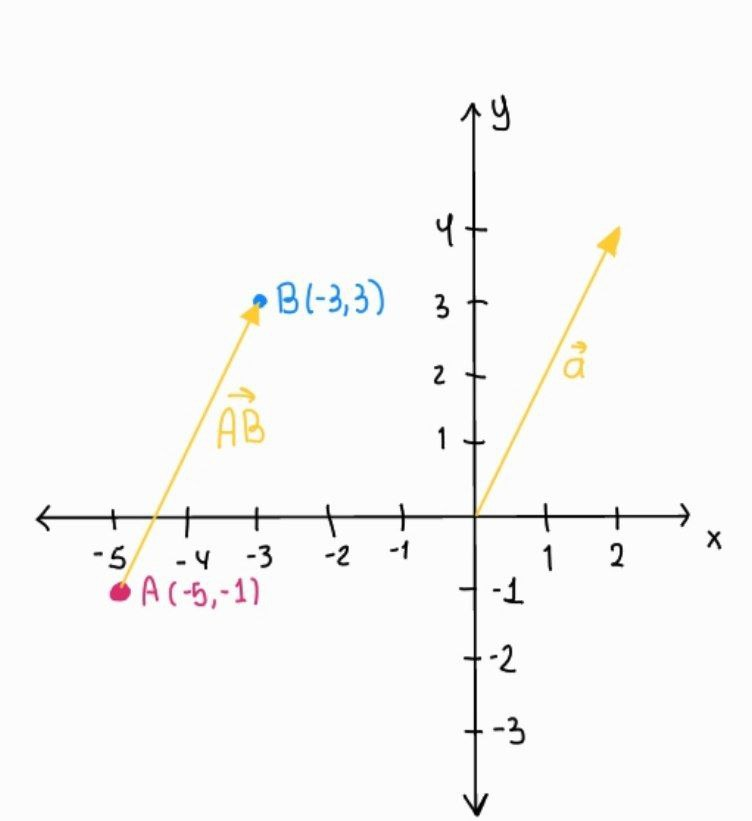
\includegraphics[width=1\textwidth]{./img/vecr2.jpeg}
  \end{figure}
\\

\item $A(0,6,1), B(3,4,4)$

  El vector correspondiente a $\vec{AB}$ es

  \begin{align*}
    \vec{a}
    &=
    \langle
    (3-0),
    (4-6),
    (4-1)
    \rangle \\
    &=
    \langle
    3,
    -2,
    3
    \rangle \\
  \end{align*}

  $\therefore \vec{a} = \langle 3, -2, 3 \rangle$
  \begin{figure}[H]
    \centering
    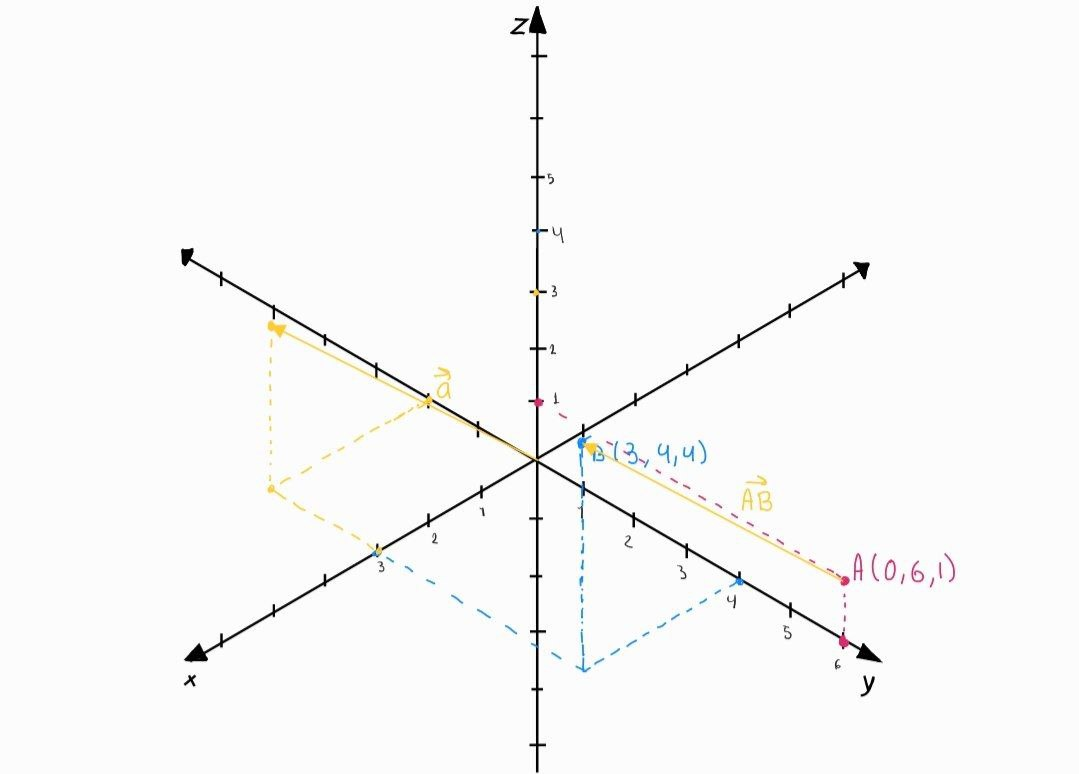
\includegraphics[width=1\textwidth]{./img/vecr3.jpeg}
  \end{figure}

\end{itemize}



% 7 -------------------------------------------------------------------------------------------------------------
\section{}

Determine:

\begin{enumerate}[format=\textbf]
  
\item $\vec{a} + \vec{b}$
  
\item $4 \vec{a} + 2\vec{b}$

\item $||\vec{a} - \vec{b}||$

\item $||\vec{a}||$

\end{enumerate}

donde $\vec{a}=8\hat{i} + \hat{j} - 4\hat{k}; \vec{b}= 5\hat{i} - 2\hat{j} +\hat{k}$ \\

Las definiciones que usaremos en este ejercicio serán las siguientes

Dados dos vectores:

\[ \vec{a} = (a_1, a_2, a_3) \]
\[ \vec{b} = (b_1,b_2, b_3) \]

y sea $c \in \mathds{R}$

\begin{itemize}
  
\item \textbf{Suma:} $\vec{a} + \vec{b}  = (a_1 + b_1, a_2+b_2, a_3+b_3)$
  
\item \textbf{Multiplicación por un escalar:} $c\vec{a} = (ca_1, ca_2, ca_3)$
  
\item \textbf{Norma:} $||\vec{a}|| = \sqrt{a_1^2 + a_2^2 + a_3^2}$
  
\item \textbf{Resta:}  $\vec{a} - \vec{b} = \vec{a} + (-\vec{b})$
  
\item \textbf{Vectores unitarios:} $\hat{i} = (1, 0, 0),  \hat{j} = (0, 1, 0),  \hat{k} = (0, 0, 1)$

\end{itemize}

En este caso, podemos reescribir los vectores dados en su forma unitario de la siguiente forma:

\[
\vec{a} = 8\hat{i} + \hat{j} - 4\hat{k} = 8(1, 0, 0) + (0,1,0) + (-4) (0,0,1) = (8, 1, -4)
\]

\[
\vec{b} = 5\hat{i} - 2\hat{j} +\hat{k} = 5(1, 0, 0) + (-2) (0,1,0) + (0,0,1) = (5, -2, 1)
\]

\begin{enumerate}[format=\textbf]
  
\item $\vec{a} + \vec{b}$
  
  \begin{equation*}
    \begin{split}
      \vec{a} + \vec{b} &= (8, 1, -4) + (5, -2, 1)\\
      &= (8+5,1+ (-2), -4+1) \\
      &=(13, 1-2, -3)\\
      &= (13, -1, -3) \\
      &= 13\hat{i} - \hat{j} -3\hat{k}
    \end{split}
  \end{equation*}
  
\item $4 \vec{a} + 2\vec{b}$
  
  \begin{equation*}
    \begin{split}
      4 \vec{a} + 2\vec{b} &= 4(8, 1, -4) + 2(5, -2, 1)\\
      &=  (32, 4, -16) + (10, -4, 2)\\
      &=  (32+10, 4-4, -16+2) \\
      &= (42, 0, -14)\\
      &= 42\hat{i}  - 14\hat{k} \\
    \end{split}
  \end{equation*}

\item $|\vec{a} - \vec{b}|$
  
  \begin{equation*}
    \begin{split}
      ||\vec{a} - \vec{b}|| &= ||(8, 1, -4) - (5, -2, 1)|| \\
      &= ||(8-5, 1-(-2), -4-1) || \\
      &= ||(3, 3, -5)|| \\
      &= \sqrt{3^2 + 3^2 + (-5)^2} \\
      &= \sqrt{9 + 9 + 25} \\
      &= \sqrt{43} \\
    \end{split}
  \end{equation*}

\item $||\vec{a}||$
  
  \begin{equation*}
    \begin{split}
      ||\vec{a}|| &= ||(8, 1, -4)|| \\
      &= \sqrt{8^2 + 1^2 + (-4)^2} \\
      &= \sqrt{64 + 1 + 16} \\
      &= \sqrt{81} \\
      &= 9
    \end{split}
  \end{equation*}
  
\end{enumerate}

% 8 -------------------------------------------------------------------------------------------------------------
\section{}

Sea $\vec{a}$ un vector tal que se ubica en el primer cuadrante, hace un ángulo de $\frac{\pi}{6}$ con el eje $x$ positivo  y $|\vec{a}|=2$. Determine $\vec{a}$ en términos de sus componentes. \\

Podemos expresar sus componentes en términos de las funciones trigonométricas, donde

\begin{align*}
  a_x​
  &= |\vec{a}| \cdot \cos{\theta} 
  = 2 \cdot \cos{\frac{\pi}{6}} 
  = 2 \cdot \left( \frac{\sqrt{3}}{2} \right) 
  = \sqrt{3} \\
  a_y
  &= |\vec{a}| \cdot \sin{\theta} 
  = 2 \cdot \sin{\frac{\pi}{6}} 
  = 2 \cdot \left( \frac{1}{2} \right) 
  = 1 
\end{align*}

$\therefore \vec{a} = \langle \sqrt{3}, 1 \rangle$

% 9 -------------------------------------------------------------------------------------------------------------
\section{}

Un vendedor ambulante vende $a$ hamburguesas, $b$ hot dogs y $c$ refrescos en un día dado. Cobra 4 pesos por hamburguesas, 2.5 pesos por hot dog y 1 peso por refresco. Sea $\vec{a}=(a,b,c)$ y $\vec{P}=(4,2.5,1)$. ¿Qué representa el producto punto $\vec{a} \cdot \vec{P}$. \\

Considerando que el producto punto entre dos vectores $\vec{u} = (u_1, u_2, u_3)$ y  $\vec{v} = (v_1, v_2, v_3)$ se define como $\vec{u} \cdot \vec{v} = u_1v_1 + u_2v_2+u_3v_3$. El producto punto  $\vec{a} \cdot \vec{P} = 4a+ 2.5b+1c$.

Sustituyendo las variables a, b, c, y los costos se interpreta como:
$\vec{a} \cdot \vec{P}$ = (Precio de una hamburguesa)(Hamburguesas vendidas)+ (Precio de un hot dog)(Hot dogs vendidos)+ (Precio de un refresco)(Refrescos vendidos).

Por lo que es fácil reconocer que $\vec{a} \cdot \vec{P}$ representa la ganancia del vendedor ambulante en un día dado.


% 10 ------------------------------------------------------------------------------------------------------------
\section{}

Encuentre las proyecciones escalar y vectorial de $\vec{b}$ sobre $\vec{a}$

\begin{itemize}
  
\item $\vec{a}= (5,12), \vec{b}=(4,6)$

  \begin{enumerate}[format=\textbf]

  \item \textbf{Proyección escalar}

    Puesto que $||\vec{a}|| = \sqrt{(5)^2 + (12)^2} = \sqrt{25 + 144} = \sqrt{169} = 13$, las proyección escalar de $\vec{b}$ sobre $\vec{a}$ es

    \begin{align*}
      comp_{\vec{a}}\vec{b}
      = \frac{\vec{a} \cdot \vec{b}}{||\vec{a}||}
      = \frac{(5 \cdot 4) + (12 \cdot 6)}{13}
      = \frac{20 + 72}{13}
      = \frac{92}{13}
      = 4
    \end{align*}

    $\therefore comp_{\vec{a}}\vec{b} = 4$

  \item \textbf{Proyección vectorial}

    La proyección vectorial es esta proyección escalar multiplicada por el vector unitario en la dirección de $\vec{a}$

    \begin{align*}
      proj_{\vec{a}}\vec{b}
      = \left( comp_{\vec{a}}\vec{b} \right) \frac{\vec{a}}{||\vec{a}||}
      = 4 \cdot \frac{\langle 5, 12 \rangle}{13}
      = \left\langle \frac{20}{13}, \frac{48}{13} \right\rangle
    \end{align*}

    $\therefore proj_{\vec{a}}\vec{b} = \left\langle \frac{20}{13}, \frac{48}{13} \right\rangle$
    
  \end{enumerate}
  
\item $\vec{a}= (1,4), \vec{b}=(2,3)$

  \begin{enumerate}[format=\textbf]

  \item \textbf{Proyección escalar}

    Puesto que $||\vec{a}|| = \sqrt{(1)^2 + (4)^2} = \sqrt{1 + 16} = \sqrt{17}$, las proyección escalar de $\vec{b}$ sobre $\vec{a}$ es

    \begin{align*}
      comp_{\vec{a}}\vec{b}
      = \frac{\vec{a} \cdot \vec{b}}{||\vec{a}||}
      = \frac{(1 \cdot 2) + (4 \cdot 3)}{\sqrt{17}}
      = \frac{2 + 12}{\sqrt{17}}
      = \frac{14}{\sqrt{17}}
    \end{align*}

    $\therefore comp_{\vec{a}}\vec{b} = \frac{14}{\sqrt{17}}$

  \item \textbf{Proyección vectorial}

    La proyección vectorial es esta proyección escalar multiplicada por el vector unitario en la dirección de $\vec{a}$

    \begin{align*}
      proj_{\vec{a}}\vec{b}
      = \left( comp_{\vec{a}}\vec{b} \right) \frac{\vec{a}}{||\vec{a}||}
      = \left( \frac{14}{\sqrt{17}} \right) \frac{\langle 1, 4 \rangle}{\sqrt{17}}
      = \left( \frac{14}{17} \right) \langle 1, 4 \rangle
      = \left\langle \frac{14}{17}, \frac{56}{17} \right\rangle
    \end{align*}

    $\therefore proj_{\vec{a}}\vec{b} = \left\langle  \frac{14}{17}, \frac{56}{17} \right\rangle$
    
  \end{enumerate}
  
\end{itemize}

% 11 ------------------------------------------------------------------------------------------------------------
\section{}

Dado los vectores $\vec{a} = \hat{i} + 2\hat{j}-2\hat{k}, \vec{b} = 4\hat{i} -3\hat{k}$

Calcule el ángulo entre los vectores:

\begin{itemize}

\item En grados

\item En radianes

\end{itemize}

Primero hay que recordar que la definición geométrica del producto punto entre dos vectores $\vec{u} = (u_1, u_2, u_3)$ y  $\vec{v} = (v_1, v_2, v_3)$ se define como  $\vec{u} \cdot \vec{v} = ||\vec{u} || \vec{v}|| \cos{\theta}$, donde $\theta$ es el ángulo formado entre $\vec{u}$ y $\vec{v}$  por lo que se sigue que:

\[
\theta = cos^{-1 }\left(\frac{\vec{u} \cdot \vec{v}}{||\vec{u}|| ||\vec{v}||}\right)
\]

Primero reescribiremos $\vec{a}$ y $\vec{b}$

\[
\vec{a} =  \hat{i} + 2\hat{j}-2\hat{k} = (1, 2, -2)
\]
\[
\vec{b} =4\hat{i} -3\hat{k}= (4, 0, -3)
\]

Calculamos el producto punto con la definición  $\vec{u} \cdot \vec{v} = u_1v_1 + u_2v_2+u_3v_3$.

\begin{equation*}
  \begin{split}
    \vec{a} \cdot \vec{b}  &= (1, 2, -2) \cdot  (4, 0, -3)  \\
    &= 4 \cdot 1 + 2 \cdot 0 + (-2) \cdot (-3) \\
    &= 4 + 0 +6 \\
    &= 10 
  \end{split}
\end{equation*}

Calculamos la norma de ambos vectores con la definición $ ||\vec{u}|| = \sqrt{u_1^2 + u_2^2 + u_3^2} $

\begin{equation*}
  \begin{split}
    ||\vec{a}||  &= ||(1, 2, -2)||  \\
    &= \sqrt{1^2 + 2^2 + (-2)^2} \\
    &= \sqrt{1 + 4 + 4} \\
    &= \sqrt{9} \\
    &=3
  \end{split}
\end{equation*}

\begin{equation*}
  \begin{split}
    ||\vec{b}||  &= ||(4, 0, -3))||  \\
    &= \sqrt{4^2 + 0^2 + (-3)^2} \\
    &= \sqrt{16 + 0 + 9} \\
    &= \sqrt{25} \\
    &= 5
  \end{split}
\end{equation*}

Sustituimos en la fórmula

\begin{equation*}
  \begin{split}
    \theta &= cos^{-1 }\left(\frac{\vec{a} \cdot \vec{b}}{||\vec{a}|| ||\vec{b}||}\right) \\
    &=  cos^{-1 }\left(\frac{10}{3 \cdot 5} \right) \\
    &= cos^{-1 }\left(\frac{10}{15} \right) \\
    &= cos^{-1 }\left(\frac{2}{3} \right) \\
  \end{split}
\end{equation*}

Y  calculamos $\theta$ :

\begin{itemize}
  
\item En grados : 48.1896851
  
\item En radianes: 0.8410686706
  
\end{itemize}

% 12 ------------------------------------------------------------------------------------------------------------
\section{}

Dados los vectores

\[\vec{a} = \hat{j}+ 7\hat{k}\]

\[\vec{b} = 2\hat{i} - \hat{j}+ 4\hat{k}\]

obtenga:

\begin{itemize}

\item $\vec{c}=\vec{a} \times \vec{b}$

  Si $\vec{a} = \langle 0, 1, 7 \rangle$ y $\vec{b} = \langle 2, -1, 4 \rangle$, entonces
  
  \begin{equation*}
    \begin{split}
      \vec{c} 
      &=
      \vec{a} \times \vec{b} \\
      &=
      \begin{vmatrix}
        \hat{i} & \hat{j} & \hat{k} \\
        0 & 1 & 7 \\
        2 & -1 & 4
      \end{vmatrix} \\
      &=
      \begin{vmatrix}
        1 & 7 \\
        -1 & 4
      \end{vmatrix}
      \hat{i}
      -
      \begin{vmatrix}
        0 & 7 \\
        2 & 4
      \end{vmatrix}
      \hat{j}
      +
      \begin{vmatrix}
        0 & 1 \\
        2 & -1
      \end{vmatrix}
      \hat{k}\\
      &=
      \{(1 \cdot 4) - [7 \cdot (-1)]\}
      \hat{i}
      -
      [(0 \cdot 4) - (7 \cdot 2)]
      \hat{j}
      +
      \{[0 \cdot (-1)] - (1 \cdot 2)\}
      \hat{k} \\
      &=
          [4-(-7)]
          \hat{i}
          -
          (0-14)
          \hat{j}
          +
          (0-2)
          \hat{k} \\
      &=
          (4 + 7)
          \hat{i}
          -
          (-14)
          \hat{j}
          +
          (-2)
          \hat{k} \\
      &=
          11 \hat{i} + 14 \hat{j} - 2 \hat{k} 
    \end{split}
  \end{equation*}

  $\therefore \vec{c} = 11 \hat{i} + 14 \hat{j} - 2 \hat{k} $

\item Compruebe que $\vec{c}$ es ortogonal a $\vec{a}$ y $\vec{b}$ simultáneamente.

  A fin de demostrar que $\vec{c} = \vec{a} \times \vec{b}$ es ortogonal a $\vec{a}$, calculamos su producto punto como sigue:
  
  \begin{equation*}
    \begin{split}
      \vec{c} \cdot \vec{a}
      &= (11 \cdot 0) + (14 \cdot 1) +[(-2) \cdot 7] \\
      &= 0 + 14 + (-14) \\
      &= 14 - 14 \\
      &= 0
    \end{split}
  \end{equation*}

  A fin de demostrar que $\vec{c} = \vec{a} \times \vec{b}$ es ortogonal a $\vec{b}$, calculamos su producto punto como sigue:
  
  \begin{equation*}
    \begin{split}
      \vec{c} \cdot \vec{b}
      &= (11 \cdot 2) + [14 \cdot (-1)] + [(-2) \cdot 4] \\
      &= 22 + (-14) + (-8) \\
      &= 22-14-8 \\
      &= 0
    \end{split}
  \end{equation*}

  $\therefore \vec{c}$ es ortogonal a $\vec{a}$ y $\vec{b}$ simultáneamente.

\end{itemize}

% 13 ------------------------------------------------------------------------------------------------------------
\section{}

Proporcione:

\begin{enumerate}

\item La ecuación vectorial

\item Las ecuaciones paramétricas

\item Las ecuaciones simétricas
  
\end{enumerate}

Para las siguientes rectas:

\begin{itemize}
  
\item La recta que pasa por $P(6,-5,2)$ y que es paralela al vector $\vec{u}=(1,3,\frac{-2}{3})$
  
\item La recta que pasa por $A(0,0,0)$ y $B(4,3,-1)$
  
\end{itemize}

Usaremos las siguientes definiciones:

\begin{itemize}
  
\item \textbf{Ecuación vectorial:} Una recta L en el espacio tridimensional se puede determinar cuando se conoce un punto $P_0(x_0, y_0, z_0)$ sobre L y la dirección de L(dada por un vector $\vec{v}$ paralelo a L).
  
  Entonces, sea $P(x, y, z)$ un punto arbitrario sobre L, sean $r_0$ y $r$ los vectores de posición de $P_0$ y $P$ y sea t un escalar.
  
  $$\vec{r} = \vec{r_0} + t\vec{v}$$
  
  es una ecuación vectorial de L, donde cada valor del parámetro t da el vector de posición r de un punto sobre L.
  Esta ecuación también se puede escribir como
  
  $$ (x, y, z) = (x_0+ta, y_0+tb, z_0+tc)$$
  
\item \textbf{Ecuación paramétrica:} La ecuaciones paramétricas de la recta L se tienen a partir de las componentes de la ecuación vectorial del inciso pasado que serían:
  $$x = x_0 + at$$
  $$y = y_0 + bt$$
  $$z = z_0 + ct$$
  
\item \textbf{Ecuación simétrica:}Esta es otra forma de describir a la recta L al eliminar el parámetro t de las ecuaciones paramétricas resolviendo para t en caso de que a, b y c sean diferentes de 0.
  
  \[
  \frac{x-x_0}{a} = \frac{y-y_0}{b} = \frac{z-z_0}{c}
  \]
  
\end{itemize}

Con estas definiciones podemos resolver los solicitado:

\begin {itemize}
  
\item La recta que pasa por $P(6,-5,2)$ y que es paralela al vector $\vec{u}=(1,3,\frac{-2}{3})$
  
  \begin{enumerate}[format=\textbf]
    
  \item Ecuación vectorial:
    
    En este caso, sea el origen O(0,0,0) $\vec{r_0} = \vec{OP} = (6, -5, 2)$  y  $\vec{v} = \vec{u} = (1,3,\frac{-2}{3})  $ y $t \in \mathds{R} $
    
    \begin{equation*}
      \begin{split}
        r &= r_0 + tv \\
        &= (6, -5, 2)  + t(1,3,\frac{-2}{3}) \\
        &= (6, -5, 2)  + (t,3t,\frac{-2}{3}t)\\
        &= (6+t, -5+3t, 2 + \frac{-2}{3}t)
      \end{split}
    \end{equation*}
    
  \item Ecuaciones paramétricas:
    
    $$x = 6+t $$
    $$y = -5+3t$$
    $$z =  2 + \frac{-2}{3}t $$
    
  \item Ecuaciones simétricas:
    
    \begin{equation*}
      \begin{split}
        \frac{x-x_0}{a} = \frac{y-y_0}{b} = \frac{z-z_0}{c} \\
        \frac{x-6}{1} = \frac{y+5}{3} = \frac{z-2}{\frac{-2}{3}} \\
        x-6 = \frac{y+5}{3} = -\frac{3}{2}(z-2) \\
      \end{split}
    \end{equation*}
    
  \end{enumerate}
  
\end{itemize}

\begin {itemize}
  
\item La recta que pasa por $A(0,0,0)$ y $B(4,3,-1)$
  
  \begin{enumerate}[format=\textbf]
    
  \item Ecuación vectorial :
    
    En este caso, sea O(0,0,0) el origen,  $\vec{r_0} = \vec{OA} = (0, 0, 0)$  y  $\vec{v} = \vec{AB}= (4,3,-1)$ y $t \in \mathds{R} $
    
    \begin{equation*}
      \begin{split}
        r &= r_0 + tv \\
        &= (0, 0, 0)  + t(4,3,-1) \\
        &= (0, 0, 0)  + (4t,3t,-t)\\
        &= (4t,3t,-t)
      \end{split}
    \end{equation*}
    
  \item Ecuaciones paramétricas:
    
    $$x = 4t $$
    $$y = 3t$$
    $$z =  -t $$
    
  \item Ecuaciones simétricas:
    
    \begin{equation*}
      \begin{split}
        t = \frac{x}{4} = \frac{y}{3} = -z
      \end{split}
    \end{equation*}
    
  \end{enumerate}
  
\end{itemize}

% 14 ------------------------------------------------------------------------------------------------------------
\section{}

Utilice el \textbf{triple producto escalar} (producto mixto) para determinar si los puntos $A(1,3,2) , B(3,-1,6), C(5,2,0), D(3,6,-4)$ son coplanares. \\

Consideremos a los siguientes vectores

\begin{itemize}

\item $\vec{a} = \vec{AB} = \langle (3-1), (-1-3), (6-2) \rangle = \langle 2, -4, 4 \rangle$

\item $\vec{b} = \vec{AC} = \langle (5-1), (2-3), (0-2) \rangle = \langle 4, -1, -2 \rangle$

\item $\vec{c} = \vec{AD} = \langle (3-1), (6-3), (-4-2) \rangle = \langle 2, 3, -6 \rangle$
  
\end{itemize}

Para determinar si son coplanares utilizamos el triple producto escalar $\vec{a} \cdot (\vec{b} \times \vec{c})$ y verificamos que sea igual a cero. Calculamos
   
\begin{equation*}
  \begin{split}
    \vec{a} \cdot (\vec{b} \times \vec{c})
    &=
    \begin{vmatrix}
      2 & -4 & 4 \\
      4 & -1 & -2 \\
      2 & 3 & -6
    \end{vmatrix} \\
    &=
    2
    \begin{vmatrix}
      -1 & -2 \\
      3 & -6 
    \end{vmatrix}
    -
    (-4)
    \begin{vmatrix}
      4 & -2 \\
      2 & -6 
    \end{vmatrix}
    +
    4
    \begin{vmatrix}
      4 & -1 \\
      2 & 3 
    \end{vmatrix}\\
    &=
    2
    \begin{vmatrix}
      -1 & -2 \\
      3 & -6 
    \end{vmatrix}
    +
    4
    \begin{vmatrix}
      4 & -2 \\
      2 & -6 
    \end{vmatrix}
    +
    4
    \begin{vmatrix}
      4 & -1 \\
      2 & 3 
    \end{vmatrix}\\
    &=
    2[(-1)(-6)-(-2)(3)]
    +
    4[(4)(-6)-(-2)(2)]
    +
    4[(4)(3)-(-1)(2)]\\
    &=
    2(6+6)
    +
    4(-24+4)
    +
    4(12+2) \\
    &=
    24 - 80 + 56 \\
    &=
    0
  \end{split}
\end{equation*}

$\therefore$ Los puntos $A(1,3,2) , B(3,-1,6), C(5,2,0), D(3,6,-4)$ son coplanares.

% 15 ------------------------------------------------------------------------------------------------------------
\section{}

Proporcione la ecuación del plano que pasa por $A(5,3,5)$y cuyo vector normal es $\vec{n}=2\hat{i} + \hat{j} - \hat{k}$. Adjunte una imagen de geogebra en la situación. \\

Usaremos la definición de \textbf{ecuación del plano}:

Un plano en el espacio se determina por un punto $P_0(x_0, y_0, z_0)$ en el plano y un vector $\vec{n}=(a,b,c)$ llamado vector normal que es ortogonal al plano. Sea P(x, y, z) un punto arbitrario en el plano y sean $r_0 = (x_0, y_0, z_0)$ y $r = (x, y,z)$ los vectores de posición de $P_0$ y $P$. Considerando que n es ortogonal a todo vector en el plano, en particular n es ortogonal a $r-r_0$.Por lo tanto se tiene:

La ecuación vectorial del plano:

\[
\vec{n} \cdot (\vec{r} - \vec{r_0}) = 0
\]

o

\[
\vec{n} \cdot \vec{r} = \vec{n} \cdot \vec{r_0}
\]

y la ecuación escalar del plano:

\[
a(x-x_0) + b(y-y_0)+c(z-z_0) = 0
\]

Entonces, la ecuación en este caso donde $\vec{n} = \vec{n}=2\hat{i} + \hat{j} - \hat{k} = (2, 1, -1)$ y $\vec{r_0}= \vec{OA} = (5,3,5)$. Entonces podemos sustituir en la ecuación escalar $a=2$, $b=1$, $c=-1$ y $x_0=5$, $y_0=3$ y $z_0=5$.

\[
2(x-5) + 1(y-3)+(-1)(z-5) = 0
\]

\[
2(x-5) +(y-3)-(z-5) = 0
\]

\[
2x-10 +y-3-z+5 = 0
\]

\[
\therefore \text{La ecuación del plano es: } 2x+y-z-8 = 0
\]

En geogebra se ve de la siguiente manera:

\begin{figure}[H]
  \centering
  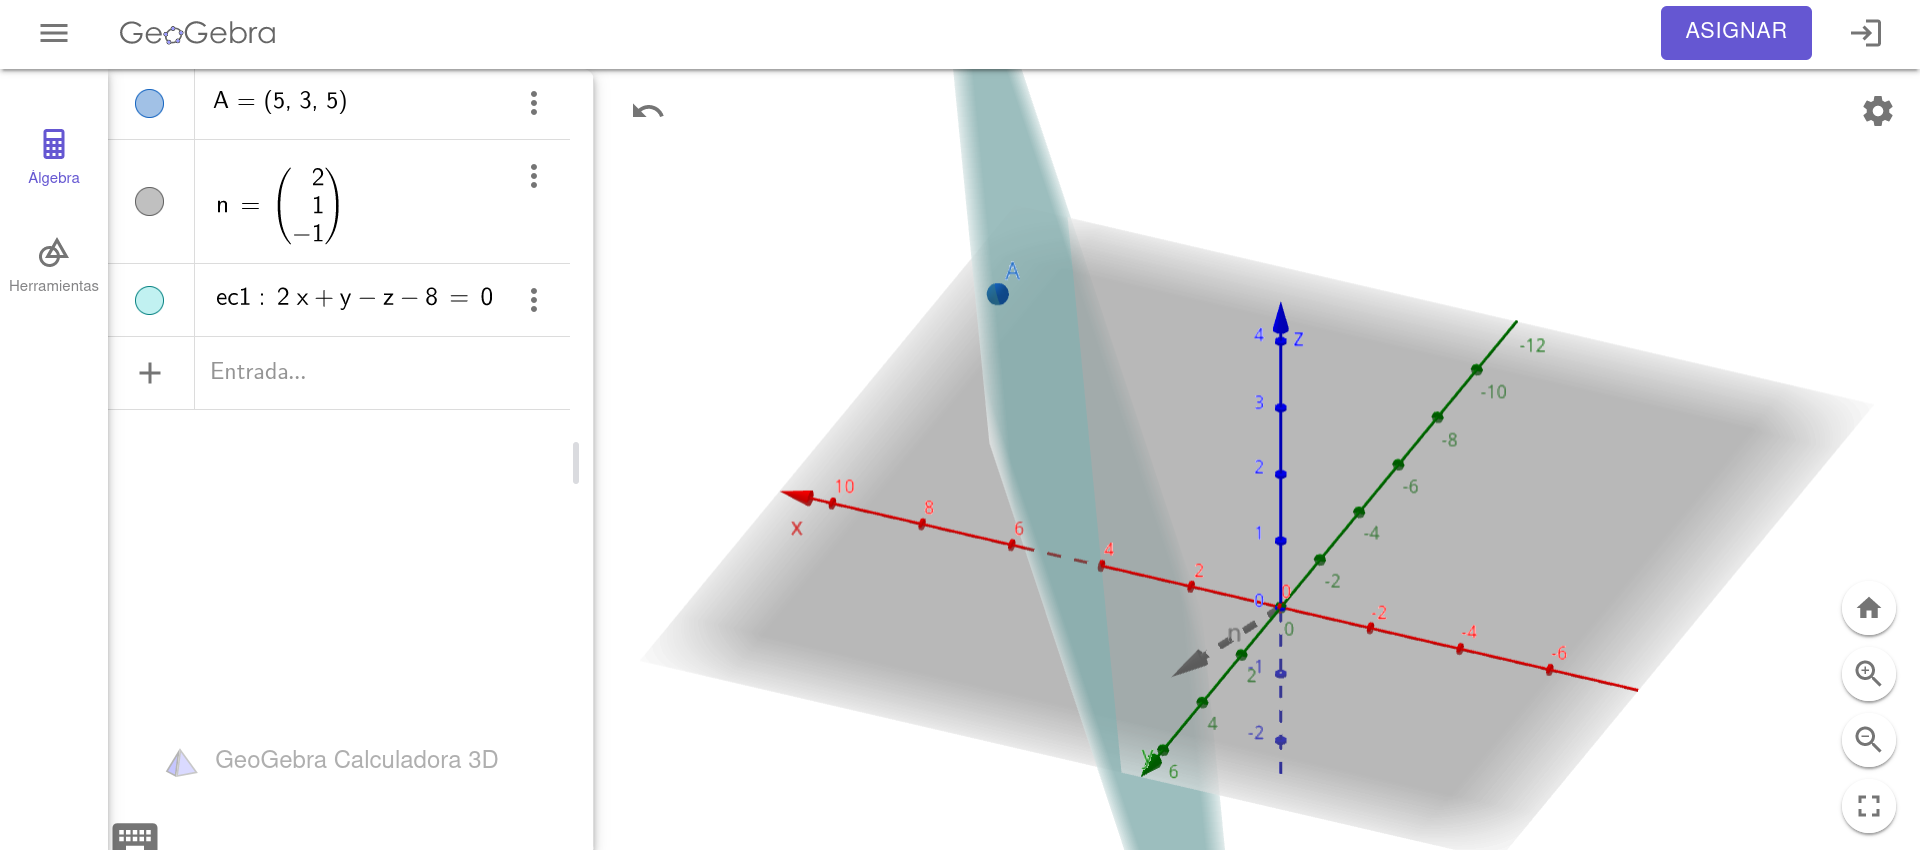
\includegraphics[width=1\textwidth]{./img/planoEc.png}
\end{figure}

% 16 ------------------------------------------------------------------------------------------------------------
\section{}

Proporcione la ecuación del plano que contiene a los puntos $A(0,0,0) , B(2,-4,6), C(5,1,3)$. Adjunte una imagen de geogebra en la situación. \\

Sean $\vec{a}$ y $\vec{b}$ los vectores que corresponden a $\vec{AB}$ y $\vec{BC}$, tenemos que

\begin{align*}
  \vec{a} &= \langle 2-0, -4-0, 6-0 \rangle \\
  &= \langle 2,-4,6 \rangle \\
  \vec{b} &= \langle 5-0, 1-0, 3-0 \rangle \\
  &= \langle 5,1,3 \rangle
\end{align*}

Puesto que $\vec{a}$ y $\vec{b}$ están en el plano, su producto cruz $\vec{a} \times \vec{b}$ es ortogonal al plano y se puede tomar como el vector normal. Así,

\begin{equation*}
  \begin{split}
    \vec{n} = \vec{a} \times \vec{b}
    &= 
    \begin{vmatrix}
      \hat{i} & \hat{j} & \hat{k} \\
      2 & -4 & 6 \\
      5 & 1 & 3
    \end{vmatrix} \\
    &=
    \begin{vmatrix}
      -4 & 6 \\
      1 & 3
    \end{vmatrix}
    \hat{i}
    -
    \begin{vmatrix}
      2 & 6 \\
      5 & 3
    \end{vmatrix}
    \hat{j}
      +
      \begin{vmatrix}
        2 & -4 \\
        5 & 1
      \end{vmatrix}
      \hat{k}\\
      &=
      [(-4)(3)-(6)(1)]
      \hat{i}
      -
      [(2)(3)-(6)(5)]
      \hat{j}
      +
      [(2)(1)-(-4)(5)]
      \hat{k}\\
      &=
      (-12-6)\hat{i}
      -
      (6-30)\hat{j}
      +
      (2+20)\hat{k}\\
      &=
      -18\hat{i}
      +24\hat{j}
      +22\hat{k}
  \end{split}
\end{equation*}

Ya que tenemos un punto $A(0,0,0)$ por el que pasa el plano, con vector normal $\vec{n}=(-18,24,22)$. Podemos sustituir estos valores en la \textbf{ecuación escalar del plano} $$a(x-x_0)+b(y-y_0)+c(z-z_0)=0$$

\begin{align*}
  -18(x-0)+24(y-0)+22(z-0)&=0 \\
  -18x+24y+22z&=0\\
  18x-24y-22z&=0\\
  9x-12y-11z&=0
\end{align*}

$\therefore$ La ecuación del plano que contiene a los puntos $A(0,0,0) , B(2,-4,6), C(5,1,3)$ es $$9x-12y-11z=0$$

\begin{figure}[H]
  \centering
  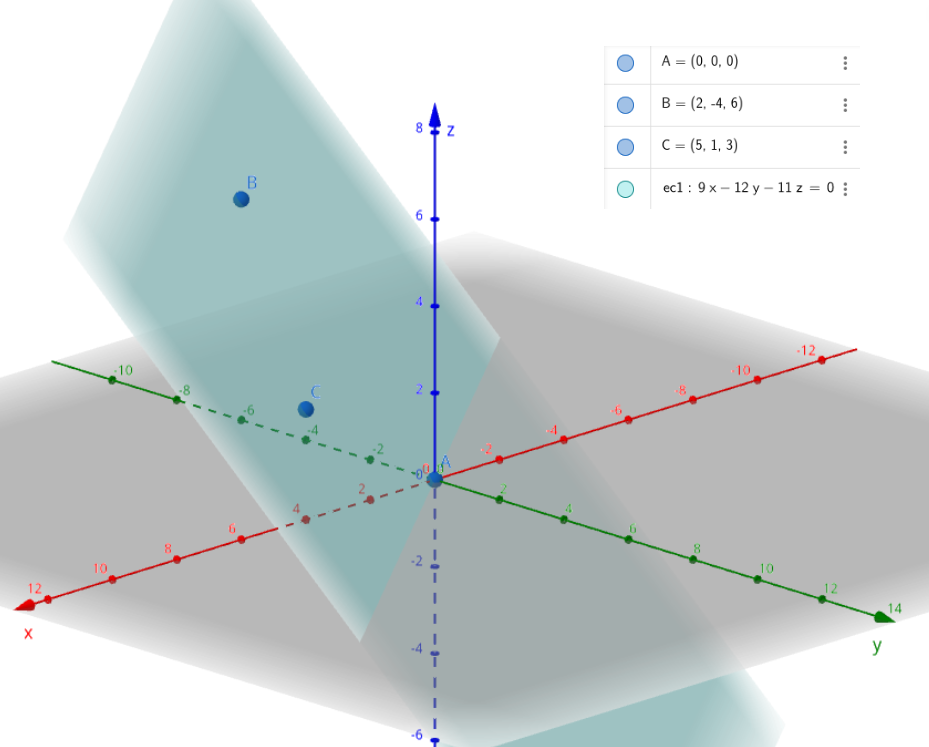
\includegraphics[width=1\textwidth]{./img/16_t1.png}
\end{figure}

% 17 ------------------------------------------------------------------------------------------------------------
\section{}

Proporcione las coordenadas del punto $A(a_x,a_y,a_x)$ del punto donde se intersecan: \\

\textbf{el plano} \\

\[ x + 2y -z+1 =0 \]

y \textbf{la recta dada por las ecuaciones paramétricas}

\begin{align*}
  x &= 1 + 2t,\\
  y &=4t,\\
  z &= 2 - 3t
\end{align*}

Adjunte una imagen de geogebrea de la situación. \\

Sustituiremos x, y, z de las ecuaciones paramétricas dadas en la ecuación del plano dada.

\[ 1 + 2t + 2(4t) - (2-3t)+1 =0 \]
\[ 1 + 2t + 8t - 2+3t +1 =0 \]
\[  13t =0 \]
\[ t = 0\]

Por lo tanto, el punto de intersección ocurre cuando el valor del parámetro es t =0.
Entonces para cada componente:

\begin{align*}
  x &= 1 + 2t = 1\\
  y &=4t = 0,\\
  z &= 2 - 3t = 2 
\end{align*}

Y por consiguiente el punto de intersección es (1, 0, 2).

En geogebra se ve de la siguiente manera:

\begin{figure}[H]
  \centering
  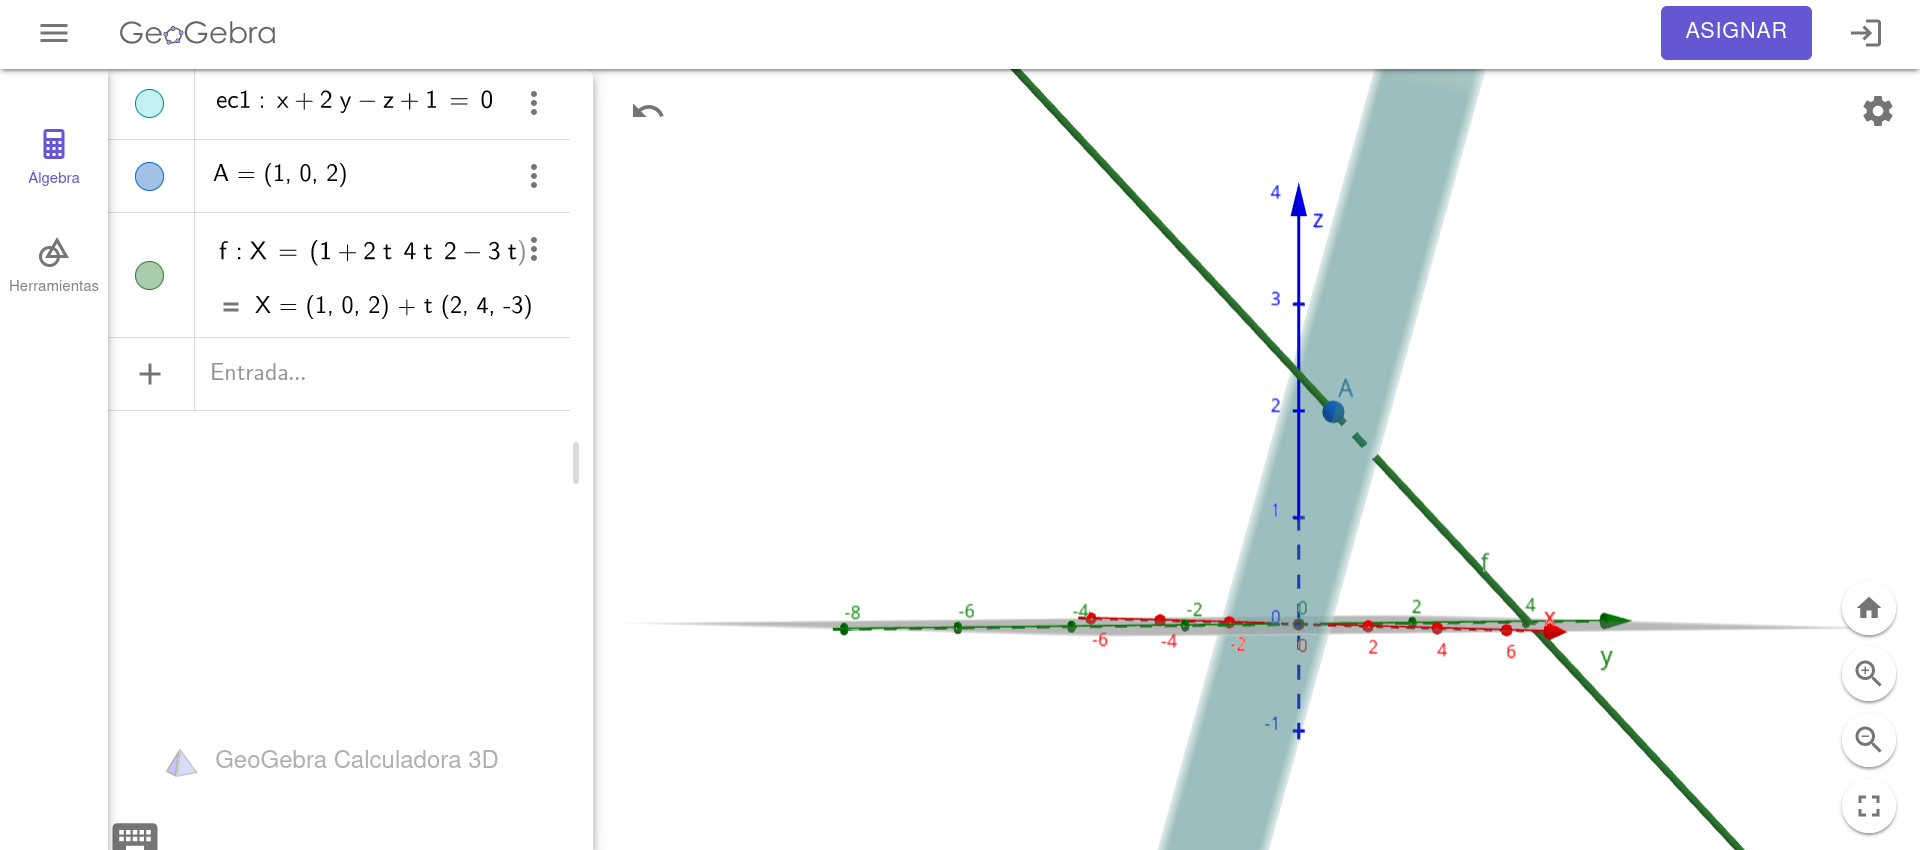
\includegraphics[width=1\textwidth]{./img/interPlano.png}
\end{figure}

\end{document}
